\documentclass[border=4pt]{standalone}
\usepackage{amsmath,amssymb,tikz}\usetikzlibrary{arrows.meta}
\definecolor{figB}{RGB}{31,90,166}\definecolor{figR}{RGB}{176,48,48}
\begin{document}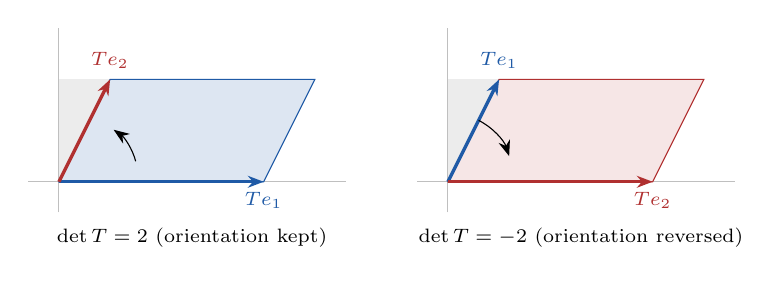
\begin{tikzpicture}[scale=1.3,>={Stealth[length=2mm]}]
\begin{scope}
\draw[gray!50] (-0.3,0)--(2.8,0) (0,-0.3)--(0,1.5);
\fill[gray!15] (0,0) rectangle (1,1); 
\fill[figB!15] (0,0)--(2,0)--(2.5,1)--(0.5,1)--cycle; \draw[figB] (0,0)--(2,0)--(2.5,1)--(0.5,1)--cycle;
\draw[->,very thick,figB] (0,0)--(2,0) node[below,font=\scriptsize]{$Te_1$};
\draw[->,very thick,figR] (0,0)--(0.5,1) node[above,font=\scriptsize]{$Te_2$};
\draw[->,thin] (0.75,0.2) arc (15:55:0.55);
\node[font=\scriptsize] at (1.3,-0.55) {$\det T=2$ (orientation kept)};
\end{scope}
\begin{scope}[xshift=3.8cm]
\draw[gray!50] (-0.3,0)--(2.8,0) (0,-0.3)--(0,1.5);
\fill[gray!15] (0,0) rectangle (1,1);
\fill[figR!12] (0,0)--(0.5,1)--(2.5,1)--(2,0)--cycle; \draw[figR] (0,0)--(0.5,1)--(2.5,1)--(2,0)--cycle;
\draw[->,very thick,figB] (0,0)--(0.5,1) node[above,font=\scriptsize]{$Te_1$};
\draw[->,very thick,figR] (0,0)--(2,0) node[below,font=\scriptsize]{$Te_2$};
\draw[->,thin] (0.3,0.6) arc (63:18:0.6);
\node[font=\scriptsize] at (1.3,-0.55) {$\det T=-2$ (orientation reversed)};
\end{scope}
\end{tikzpicture}\end{document}
